\documentclass[12pt]{report} 

% language may be romanian or english (default is english)
% type may be bachelor or master (default is bachelor)
\usepackage[language=romanian, type=bachelor]{style}

%\geometry{a4paper,top=2.5cm,left=3cm,right=2.5cm,bottom=2.5cm}
%in style
%controlling the appearance of your headers and footers
\usepackage{fancyhdr}    
\pagestyle{fancy}
\lhead{}
\chead{}
\renewcommand{\headrulewidth}{0.2pt}
\renewcommand{\footrulewidth}{0.2pt}

\begin{document}

\specialization{INFORMATICĂ ÎN LIMBA ROMÂNĂ}	
\title{Conectarea persoanelor bazată pe interese comune folosind sisteme de recomandare}					   
\author{Bucilă Mihai-Cristian}											
\supervisor{Asist. Drd. Coste Claudia-Ioana \\ Prof. univ. Dr. Andreica Anca-Mirela}				
				
\maketitle


\newpage
\thispagestyle{empty}
\mbox{}
\newpage
\pagenumbering{roman} 

\cleardoublepage
ABSTRACT
\vspace{0.5cm}	
\hrule
\vspace{0.5cm}	
%\cleardoublepage

\par
The abundance of information on the internet has driven the rapid evolution of recommender systems.
Their ability to provide personalized suggestions has led to widespread adoption in high-demand areas like e-commerce and social networking platforms, enhancing both user experience and retention.
\par
This thesis presents the core techniques underlying recommendation systems --- content-based filtering and collaborative filtering --- and explores the challenges that can arise when implementing these methods, such as the cold start problem, synonymy and privacy concerns.
The main objective of this work is to demonstrate the utility of a recommender system in the context of an application that matches users based on their shared hobbies.
The application analyzes user-provided hobby data and uses a simplified matching algorithm to identify potential matches within a shared interest space.
\par
This work is motivated by the idea that recommender systems can have an impact beyond commercial platforms and enhance social connectivity and community building.
By combining the theoretical knowledge with a concrete implementation, the project shows how recommendation techniques can be adapted to support social engagement and personal development.
The application serves not only as a case study, but also as a proof of concept for using technology to bring people together in a more intentional way.

\tableofcontents


\newpage
\pagenumbering{arabic}

\chapter{Introducere}

%\chapter*{Introducere}
\label{intro}

Hobby-ul este o activitate plăcută pe care o persoană o face regulat, cu dorința de a se relaxa. Acesta nu trebuie confundat cu profesia, deoarece nu urmărește vreun obiectiv profesional sau financiar.

\section{Motivație}
\label{section:ch1sec1}


\section{Obiective}
\label{section:ch1sec2}


\section{Structura lucrării}
\label{section:ch1sec3}

Această lucrare este structurată în 5 capitole care prezintă atât aspecte teoretice, cât și aspecte practice ale subiectului abordat. Capitolul 1 prezintă o introducere a temei propuse, cu atenția îndreptată spre obiectivele lucrării și motivația acesteia. În capitol 2 se oferă detalii despre câteva soluții existente ce rezolvă problema dată. Capitolul 3 este dedicat bazei teoretice. Soluția software se descrie în capitolul 4. În capitolul 5 sunt prezentate concluziile și perspectivele de viitor.
%\addcontentsline{toc}{chapter}{Introducere}
%\addcontentsline{toc}{chapter}{Introduction}

\chapter{Soluții similare în domeniul sistemelor de recomandare}
\label{chap:ch2}

Sistemele de recomandare sunt folosite la scară largă în multe aplicații, oferind conținut personalizat și o experientă de utilizare îmbunătățită. 
Aplicațiile ce le folosesc variază, de la platforme de comerț online la rețele sociale.
Scopul acestora este de a ajuta utilizatorii să obțină conținut relevant din cantitatea mare de informație care există, simplificând procesul de căutare.
Astfel de soluții contribuie semnificativ creșterea veniturilor companiilor și la fidelizarea utilizatorilor.
Algoritmii folosiți în astfel de sisteme sunt filtrarea bazată pe conținut, filtrarea colaborativă sau soluții hibride, fiecare cu avantajele și limitările sale.
Pe lângă preferințele redate direct de utilizatori, sistemele moderne de recomandare țin cont și de context: locație, dispozitiv folosit sau momentul zilei.
Cu toate acestea, tehnicile se confruntă cu anumite provocări, precum problema utilizatorilor noi, lipsa de diversitate în recomandări sau lipsa de transparență a algoritmilor.

\section{Platforme de vânzări}
\label{sec:ch2sec1}
\subsection*{Amazon}
Amazon este una dintre cele mai cunoscute platforme de comerț care utilizează sisteme de recomandare.
Acesti algoritmi sunt integrați în întreaga aplicație, de la pagina principală până la paginile individuale ale produselor.
Platforma folosește tehnologii avansate de recomandare și de analiză a datelor pentru a afla comportamentul utilizatorilor.
Datele relevante pentru sistem sunt: produsele vizualizate, adăugate în coș sau cumpărate, recenzii, istoricul căutărilor, dar și comportamentul altor utilizatori cu profil similar. 
Toate aceste date sunt folosite pentru a crea profiluri detaliate de utilizator, cu rol crucial în oferirea de recomandări personalizate.
Pe baza acestora, Amazon implementatează metode precum filtrarea bazată pe conținut (pentru a recomanda produse similare celor accesate în trecut) și filtrarea colaborativă (cu scopul de a sugera produse populare în rândul utilizatorilor cu interese comune).
Sistemul lor de recomandare este considerat un factor cheie în maximizarea eficienței vânzărilor, ajutând la retenția clienților și stimulând cumpărăturile recurente\cite{ahmed2022amazon, smith2017two}.

\subsection*{Netflix}
Netflix este un exemplu de serviciu de tip streaming care implementează algoritmi de recomandare pentru a îmbunătăți experiența utilizatorilor și pentru a crește nivelul de satisfacție al acestora.
Fără acest sistem, platforma nu s-ar bucura de succesul pe care îl are.
La fel ca Amazon, Netflix folosește o combinație de tehnici, adaptate pentru a oferi sugestii personalizate. 
Sistemul ia în considerare date ce privesc durata și istoricul vizionărilor, rating-ul acordat filmelor și interacțiunile anterioare.
Impactul acestor tehnologii este semnificativ, astfel că Netflix reușește să crească timpul petrecut în aplicație și să mărească gradul de fidelizare a utilizatorilor.
Mai mult, recomandările ajută abonații să descopere titluri noi, pe care probabil nu le-ar fi căutat, sporind aprecierea lor pentru platformă\cite{chiny2022netflix, gomez2015netflix}.

\section{Rețele sociale}
\label{sec:ch2sec2}
\subsection*{Facebook}
Facebook este una dintre cele mai utilizate rețele sociale la nivel mondial.
Sistemele de recomandare sunt esențiale în modul în care platforma afișează noutățile, sugerează prieteni sau grupează pagini relevante pentru fiecare persoană.
Algoritmii aplicației analizează numeroși factori precum interacțiunile anterioare (reacții, comentarii, distribuiri), timpul petrecut pe anumite tipuri de postări, relațiile dintre utilizatori, dar și preferințele implicite, deduse din comportament.
Aceste informații sunt prelucrate în timp real pentru a determina ce conținut este cel mai relevant. 
Se poate observa că acest mod de personalizare influențează modul în care utilizatorii percep realitatea digitală, întrucât conținutul afișat este filtrat și ordonat în funcție de relevanță, nu de cronologie sau obiectivitate\cite{baatarjav2008group}.
\par
Un alt aspect important este faptul că platforma nu oferă doar recomandări explicite (sugestii de prieteni sau grupuri), ci și implicite, prin modul în care organizează și filtrează fluxul de informații. 
Acestea optimizează și afișarea reclamelor, asigurând o potrivire mai bună între interesele utilizatorilor și ofertele companiilor, mărind astfel eficiența campaniilor publicitare și veniturile platformei.
Astfel, persoanele care utilizează aplicația sunt predispuse să petreacă mai mult timp explorând conținut, interacționând cu prietenii și postările acestora, ceea ce determină un nivel ridicat de implicare și angajament față de platformă.
Prin utilizarea acestor tehnologii, Facebook nu doar îmbunătățește experiența individuală, ci și crește implicarea utilizatorilor, contribuind la menținerea unei baze de date active\cite{heimbach2015value}.
\par
Cu toate acestea, folosirea excesivă a algoritmilor poate conduce la crearea unor „bule informaționale”\cite{nguyen2014exploring}, unde utilizatorii sunt expuși doar la un anumit tip de conținut, ce le confirmă convingerile existente, limitând diversitatea opiniilor și a informațiilor la care o persoană poate avea acces.
În tot acest timp, personalizarea exagerată influențează percepția asupra realității și poate reduce capacitatea de a descoperi perspective noi sau diferite.

\section{Abordări existente în conectarea utilizatorilor bazată pe interese}
\label{sec:ch2sec3}
O direcție importantă în cadrul sistemelor de recomandare este reprezentată de metode de asociere între utilizatori, în functie de interesele comune.
Aceste abordări sunt des întâlnite în aplicații de socializare, unde rolul lor este de a facilita conexiunile relevante între persoanele cu profiluri similare.
\par
În unul dintre articolele de specialitate\cite{tsakalakis2018improved}, autorii propun să abordeze problema recomandării de prietenii prin dezvoltarea unei metode avansate de calcul a similarității între utilizatori.
Obiectivul principal al algoritmului lor este de a conecta persoane cu interese comune care se află în aceeași zonă geografică.
Autorii au evaluat performanțele metodei proiectate pe un eșantion de 286 de utilizatori prin compararea lor cu alte metode clasice de calcul ale similarității existente în literatură, obținând rezultate superioare în contextul specific.
\chapter{Fundamente teoretice în sisteme de recomandare}
\label{chap:ch3}

Acest capitol prezintă fundamentele teoretice care stau la baza sistemelor de recomandare, punând accent pe metodele utilizate în practică: filtrarea bazată pe conținut și filtrarea colaborativă.
De asemenea, sunt remarcate provocările cu care aceste sisteme se confruntă, precum problema „cold start”, ambiguitățile semantice și aspecte legate de securitate și confidențialitate.
Aceste concepte teoretice oferă cadrul necesar pentru înțelegerea și dezvoltarea unui sistem de potrivire între persoane.

\section{Filtrare bazată pe conținut}
\label{sec:ch3sec1}

Filtrarea bazată pe conținut este o tehnică de recomandare care analizează atributele unui element sau ale unei persoane pentru a genera sugestii.
În general, această metodă este utilizată cu scopul de a oferi recomandări personalizate în funcție de profilul utilizatorilor.
Sistemul identifică similarități între profiluri și sugerează elemente sau persoane care corespund cel mai bine preferințelor utilizatorului\cite{kumar2018recommendation}.
\par
Această metodă este des utilizată în platforme precum Spotify, YouTube sau Netflix, în special pentru a recomanda conținut similar cu cel deja consumat. 
De exemplu, un utilizator care ascultă muzică jazz va primi mai frecvent recomandări din aceeași zonă muzicală, fără a fi nevoie de comparații cu preferințele altor utilizatori. 
Avantajul major al acestui tip de filtrare constă în caracterul său personalizat, axat strict pe gusturile fiecărui utilizator, fără a fi influențat de tendințele generale ale comunității.
\par
Cu toate acestea, filtrarea bazată pe conținut are și unele limitări. 
Una dintre cele mai notabile este lipsa diversității — sistemul poate rămâne „prizonier” în tiparele stabilite inițial și poate recomanda doar conținut foarte similar cu ceea ce a fost deja consumat. 
În plus, eficiența sistemului depinde de calitatea datelor și de granularitatea atributelor folosite pentru descrierea obiectelor.

\subsection{Principiu de funcționare}
Metoda se bazează pe construirea unui profil pentru fiecare utilizator, care reflectă preferințele sale în funcție de conținutul anterior accesat sau evaluat. 
Acest profil este comparat cu descrierile altor elemente disponibile, iar sistemul recomandă acele elemente care prezintă cele mai mari similarități.
De regulă, se folosesc tehnici de procesare a limbajului natural, metode probabilistice sau modele de învățare automată.
Una dintre particularitățile filtrării bazate pe conținut este faptul că nu are nevoie de date despre alți utilizatori pentru a funcționa. Recomandările sunt generate exclusiv pe baza preferințelor și comportamentului.
Acest lucru oferă o flexibilitate ridicată, în special atunci când predilecțiile se schimbă. Pe de altă parte, această abordare presupune existența unor descrieri detaliate ale elementelor din sistem, ceea ce poate deveni o provocare atunci când aceste informații lipsesc sau sunt dificil de structurat\cite{ISINKAYE2015261}.
\section{Filtrare colaborativă}
\label{sec:ch3sec2}
\section{Provocări și limitări ale metodelor de recomandare}
\label{sec:ch3sec3}
Deși sistemele de recomandare bazate pe conținut și colaborative au un rol esențial în personalizarea experienței utilizatorilor, acestea se confruntă cu o serie de limitări care pot afecta eficiența și precizia recomandărilor. 
Printre cele mai întâlnite provocări se numără lipsa datelor suficiente pentru utilizatorii noi, dificultatea de a surprinde preferințele în schimbare și complexitatea modelării relațiilor între elemente sau utilizatori. 
În continuare sunt prezentate câteva dintre aceste probleme, împreună cu implicațiile lor asupra performanței sistemelor de recomandare.

\subsection{Problema „Cold start”}
\label{subsec:ch3sec3sub1}
Problema „Cold start”\cite{lika2014facing} reprezintă o situație care este des întâlnită în domeniul sistemelor de recomandare. 
Aceasta apare atunci când nu există suficiente date despre un utilizator sau un obiect pentru a face recomandări precise.
În cazul unui utilizator nou, sistemul nu dispune de informații suficiente despre acesta, făcând dificilă furnizarea sugestiilor.
În mod similar, în cazul unui obiect nou, 
Astfel, se poate ajunge la recomandări inexacte ce afectează negativ experiența utilizatorului.
Soluțiile pentru această problemă includ utilizarea tehnicilor de recomandare bazate pe conținut, care nu depind de interacțiuni anterioare, 
în detrimentul recomandărilor colaborative sau combinarea mai multor metode pentru o acuratețe îmbunătățită în etapele incipiente de folosire.
Concret, sistemul ar trebui fie să ofere posibilitatea unui utilizator nou să evalueze anumite articole sau să întrebe explicit despre gusturile acestuia pentru a-i construi un profil, 
fie să dea recomandări preliminare bazate pe informații demografice sau alte date disponibile\cite{kumar2018recommendation}.


\subsection{Sinonimie și polisemie}
\label{subsec:ch3sec3sub2}
În cadrul sistemelor de recomandare, sinonimia apare atunci când doi termeni diferiți descriu același concept (de exemplu, „movie” și „film”, „football” și „soccer”).
Acești termeni sunt tratați ca entități distincte, afectând performanța recomandărilor, deoarece similaritatea latentă dintre interese nu este exploatată.
Pentru a contracara fenomenul, literatura de specialitate propune tehnici care extind vocabularul cu termeni echivalenți sau identifică automat legături între date, astfel încât acestea să fie grupate în funcție de sensul lor.
Totuși, soluțiile nu sunt perfecte, pentru că acești termeni pot avea sensuri ușor diferite față de cele intenționate și pot duce la o asociere irelevantă\cite{mansur2017review}.
\par
Pe lângă sinonimie, polisemia este o problemă similară care afectează generarea de recomandări. În acest caz, un singur termen are mai multe înțelesuri, în funcție de context, iar sistemul poate face asocieri eronate.
Aceste două probleme favorizează apariția erorilor în recomandare și evidențiază nevoia unor mecanisme semantice de interpretare a datelor care să țină cont de nuanțele limbajului natural\cite{lops2011content}.

\subsection{Confidențialitate și securitate}
\label{subsec:ch3sec3sub3}
Confidențialitatea și securitatea sunt două concepte ce vizează efectele sistemului de recomandare asupra utilizatorilor.
Dat fiind faptul că sistemele de recomandare se bazează pe colectarea și procesarea datelor sensibile, precum preferințe și istoric de vizualizare, acestea ridică probleme majore în ceea ce privește confidențialitatea și securitatea.
Păstrarea acestor date fără protecție poate conduce la scurgeri de informații, afectând eficiența sistemului și încrederea utilizatorilor\cite{huang2019privacy}.
Pentru prevenirea expunerii datelor, un articol de specialitate recomandă utilizarea unor metode criptografice avansate, precum criptarea homomorfă, care permite sistemului să recomande fără ca el să aibă acces la informația reală a utilizatorilor\cite{badsha2016practical}.
\par
Aceste măsuri nu protejează doar datele utilizatorilor în sine, ci și dezvoltă un nivel de încredere ridicat. 
Persoanele în cauză sunt sigure că datele lor nu sunt exploatate în mod negativ.
\sloppy
\chapter{Aplicație software}
\label{chap:ch4}

\par
Capitolul de față descrie aplicația software realizată, prezentând structura sa generală, principalele componente și modul în care acestea comunică pentru a oferi funcționalitățile propuse.
Sunt oferite detalii despre arhitectură și sunt explicate principalele funcționalități. 
Capitolul se încheie cu un scurt manual de utilizare, conceput să ghideze utilizatorul în folosirea aplicației. 

\section{Arhitectura aplicației}
\label{sec:ch4sec1}

Aplicația este alcătuită din 3 componente: interfața utilizator (frontend), partea de server (backend) și sistemul de recomandare. 
Partea de frontend este dezvoltată în Ionic React \cite{ionicreactdocs}, tehnologie ce îmbină librăria React \cite{reactdocs}, scrisă în limbajul de programare JavaScript, 
utilizată pentru a construi interfețe utilizator și Ionic \cite{ionicdocs}, un instrument ce ajută la dezvoltarea aplicațiilor cross-platform. 
Folosind Ionic, aplicația poate fi instalată pe mai multe platforme --- web, mobile (Android, iOS), desktop --- utilizând același cod sursă. 
Această abordare eficientizează dezvoltarea și întreținerea aplicațiilor, permițând o experiență de utilizare uniformă, indiferent de dispozitiv folosit. 

\subsection{Frontend}
\label{subsec:ch4sec1sub1}
Interfața utilizator a aplicației este compusă din rute, pagini și componente. 
Paginile corespund unor ecrane complete din aplicație, iar componentele sunt părți reutilizabile ale aplicației, precum un formular sau buton personalizat.
Componentele primesc proprietăți și returnează elemente de interfață utilizator.
Rutele definesc ce pagină trebuie afișată atunci când utilizatorul accesează o anumită adresă (URL). 
De exemplu, ruta \texttt{/login} afișează pagina de autentificare, ruta \texttt{/register} afișează pagina de înregistrare ș.a.m.d.

\par
Frontend-ul comunică cu serverul prin apeluri HTTP, datele fiind transmise în formatul JSON.
În cadrul aplicației a fost creat fișierul \texttt{api.ts} care grupează toate cererile care sunt trimise către backend. 
Acest serviciu oferă funcții precum \texttt{register}, \texttt{login} și \texttt{saveHobbies}.
Aplicația folosește biblioteca Axios, o soluție populară și eficientă pentru manipularea cererilor HTTP.


\subsection{Backend}
\label{subsec:ch4sec1sub2}
Partea de server este scrisă în Java utilizând Spring Boot \cite{springbootdocs}, un instrument care ajută la simplificarea procesului de dezvoltare al aplicațiilor.
Acest framework permite crearea rapidă de API-uri REST, o integrare facilă cu baza de date și o organizare logică a codului în componente. Alegerea
acestei tehnologii a fost motivată de ecosistemul extins pe care îl oferă, configurarea redusă și structura modulară. 

\par
Proiectul este organizat conform principiilor arhitecturii stratificate, adaptate pentru o aplicație REST. 
Așadar, codul sursă este împărțit în mai multe directoare (pachete) care separă responsabilitățile logice: 
\begin{itemize}
    \item controller: include clase care gestionează cererile HTTP venite de la frontend. Acestea definesc rutele API și interacționează direct cu serviciile.
    \item service: conține implementările operațiilor specifice fiecărei funcționalități (înregistrare utilizator, adăugare hobby etc.). Acest strat realizează legătura între controller și repository. 
    \item repository: definește interfețe care extind \texttt{JpaRepository}. Acestea se concentrează asupra operațiilor CRUD (Create, Read, Update, Delete) cu efect direct asupra bazei de date.
    \item domain: conține entitățile din domeniul aplicației. Acestea sunt adnotate cu specificații precum \texttt{@Entity}, \texttt{@Table} etc. pentru a le asocia tabelelor din baza de date.
\end{itemize}  
Pe lângă aceste pachete clasice, proiectul include și alte componente utile:
\begin{itemize} 
    \item dto (Data Transfer Object): conține clase care precizează formatul datelor transmise între client și server.
    \item mapper: cuprinde clase cu metode statice folosite la conversia obiectelor de tip domeniu în obiecte de tip DTO și vice-versa.
    \item exception: definește clase care se ocupă de tratarea erorilor. Acestea extind clasa \texttt{Exception} cu scopul de a crea excepții personalizate.
    \item security: gestionează autentificarea și autorizarea. Oferă implementare pentru JWT (Json Web Token).
\end{itemize}
\subsubsection*{Model de date}
Entitățile de bază ale aplicației sunt User, Hobby și HobbyType. Fiecare dintre acestea sunt reprezentate printr-o clasă Java, asociată unei tabele din baza de date.
În figura \ref{FigClassDiagram} sunt definite clar relațiile între obiecte.

\begin{figure}[htbp]
	\centering
    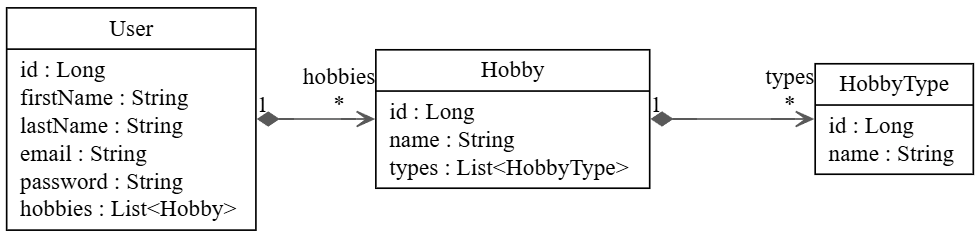
\includegraphics[scale=0.40]{./figures/class-diagram.png}
	\caption{Diagrama de clase}
	\label{FigClassDiagram}
\end{figure}

\subsubsection*{Baza de date}
Conectarea la baza de date se face cu ajutorul fișierului de configurare \texttt{application.properties}, unde sunt specificate datele de acces precum URL, utilizator și parolă. 
Baza de date folosită este PostgreSQL \cite{postgresqldocs}, consacrată pentru fiabilitate și performanță. 
Pentru asocierea obiectelor Java cu tabelele bazei de date s-a utilizat Java Persistence API împreună cu framework-ul Hibernate \cite{hibernatedocs}, permițând manipularea entităților Java ca tabele din baza de date, așa cum se poate vedea în figura \ref{FigDbDiagram}.

\begin{figure}[htbp]
	\centering
    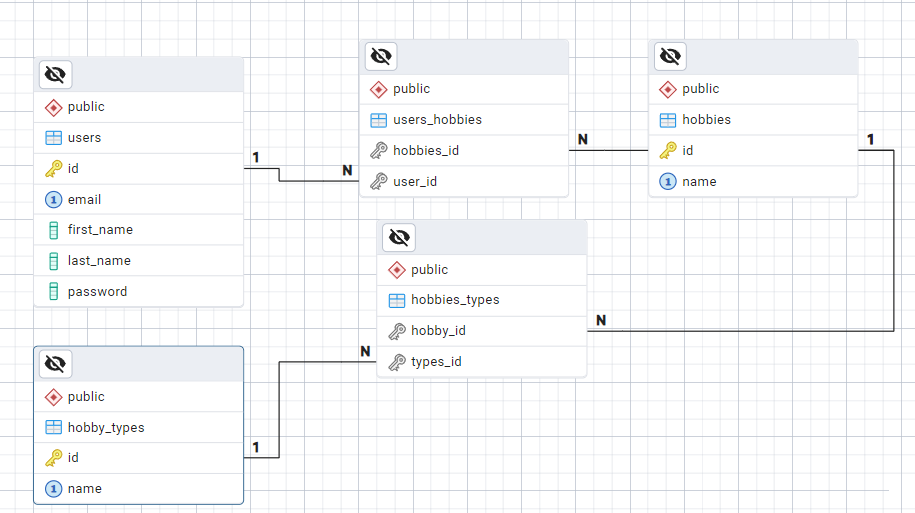
\includegraphics[scale=0.65]{./figures/db-diagram.png}
	\caption{Diagrama bazei de date}
	\label{FigDbDiagram}
\end{figure}

\subsubsection*{Securitate}
Aplicația implementează câteva mecanisme minimale de asigurare a securității și de protejare a accesului la resursele interne.
În ceea ce privește parola asociată contului, aceasta este stocată sub formă criptată, folosind algoritmul BCrypt, iar pentru siguranța parolei, aplicația impune o lungime minimă de 8 caractere a acesteia.
Atunci când utilizatorul se autentifică cu succes, primește un JSON Web Token (JWT). Acest token este folosit pentru identificarea ulterioară a utilizatorului în cererile către server.
Deoarece majoritatea rutelor din aplicație sunt restricționate, utilizatorul are nevoie de un token valid pentru a le accesa, ceea ce asigură un control al accesului la funcționalitățile interne ale aplicației.

\subsection{Sistemul de recomandare}
\label{subsec:ch4sec1sub3}
Pentru a determina gradul de similaritate între utilizatori pe baza hobby-urilor comune, sistemul folosește coeficientul de similaritate Jaccard.
Această metodă compară seturile de hobby-uri ale fiecărui utilizator și calculează raportul dintre elementele comune și totalitatea elementelor distincte din cele două seturi.
Rezultatul este un număr real între 0 și 1. Această metodă este simplă și intuitivă, fiind adecvată pentru compararea mulțimilor neordonate de termeni.
Implementarea funcției care calculeaza similaritatea Jaccard este prezentată în secvența de cod \ref{CodeJaccard}.

\begin{lstlisting}[caption={Algoritmul de calcul al similarității Jaccard}, label={CodeJaccard}]
def jaccard_similarity(set1, set2):
    if not set1 or not set2:
        return 0.0
    intersection = len(set1.intersection(set2))
    union = len(set1.union(set2))
    return intersection / union
\end{lstlisting}    

\subsubsection*{Setul de date}
Pentru a popula baza de date cu o listă de hobby-uri cât mai bogată și realistă, s-au fuzionat trei seturi de date disponibile pe platformele Kaggle \cite{kaggle_Raj, kaggle_dawid} și HuggingFace \cite{hf_Ugurcan}.
După îmbinarea acestora, a fost nevoie de o prelucrare atentă a setului de date pentru a standardiza formatul.
Numele hobby-urilor au fost normalizate, iar în cazul în care au apărut duplicate, acestea au fost eliminate, însă tipurile lor au fost comasate.
Tipurile hobby-urilor au fost la rândul lor prelucrate, deoarece erau exprimate inconsistent, separate fie prin virgulă, fie prin conjuncția ”and”, iar duplicatele au fost excluse.
În urma procesării, s-a obținut un set de aproximativ 730 de hobby-uri care a fost introdus în baza de date pentru ca utilizatorii să poată selecta hobby-urile dintr-o listă structurată.

\subsubsection*{Comunicare cu serverul Java}
Recomandările se realizează printr-o comunicare între serverul Java și sistemul de recomandare, care este implementat separat, scris în Python, folosind framework-ul Flask \cite{flaskdocs}.
Acest serviciu extern este responsabil cu procesarea datelor și calculul gradului de asemănare.
Atunci când utilizatorul accesează pagina de căutare a recomandărilor, aplicația trimite către serverul Python informații despre hobby-urile acestuia, precum și despre restul utilizatorilor existenți.
Sistemul analizează datele și returnează o listă de utilizatori cu interese comune, ordonați în funcție gradul de similaritate.
\par
Alegerea de a implementa separat acest sistem de recomandare a fost motivată de dorința de a păstra componenta independentă față de restul aplicației.
Această abordare dă posibilitatea de a reutiliza codul într-un alt context, precum recomandarea de produse, cărți sau filme.

\section{Funcționalități}
\label{sec:ch4sec2}

Aplicația se concentrează asupra a patru acțiuni esențiale: înregistrarea unui cont, autentificarea unui utilizator, selectarea hobby-urilor dorite și căutarea altor utilizatori cu hobby-uri similare.
Diagrama din figura \ref{FigUseCaseDiagram} evidențiază aceste funcționalități.

\begin{figure}[htbp]
	\centering
    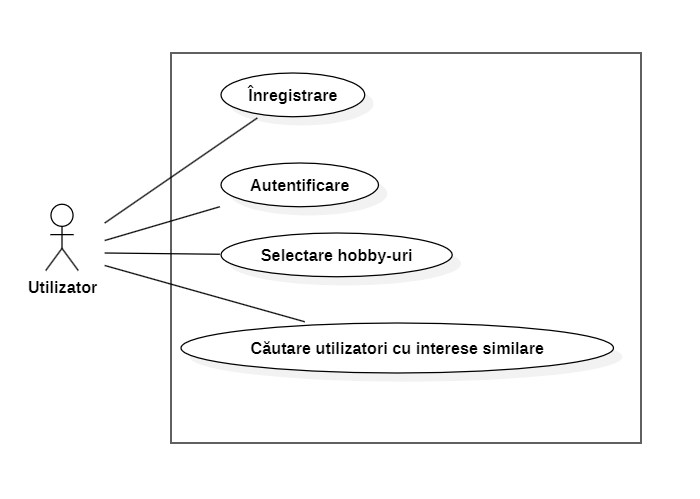
\includegraphics[scale=0.60]{./figures/usecase-diagram.png}
	\caption{Diagrama cazurilor de utilizare}
	\label{FigUseCaseDiagram}
\end{figure}

\subsection{Înregistrarea utilizatorului}
\label{subsec:ch4sec2sub1}
Această funcționalitate permite unui user nou să își creeze cont în aplicație. Pagina conține un formular cu câmpurile: nume, prenume, email sau parolă.
La acționarea butonului Register, aplicația validează datele scrise de utilizator, iar în cazul în care
nu există erori, trimite o cerere HTTP de tip POST către endpoint-ul \texttt{/auth/register} expus de backend. În caz contrar, programul oferă user-ului feedback imediat prin mesaje de eroare sugestive.
Pe backend, datele se revalidează pentru a asigura securitatea și integritatea acestora. 
Contul utilizatorul se salvează în baza de date doar dacă nu există deja unul cu aceeași adresă de email, altfel se aruncă o excepție corespunzătoare.
Serverul trimite răspuns, după caz, fie datele user-ului creat, fie un mesaj de eroare.

\subsection{Autentificarea utilizatorului}
\label{subsec:ch4sec2sub2}
Pentru a accesa restul funcționalităților, utilizatorul trebuie să se autentifice. Pagina dedicată logării cuprinde un formular cu două câmpuri: adresa de email și parolă.
În urma apăsării butonului Login, aplicația validează local datele introduse. În lipsa erorilor, se inițiază o cerere HTTP POST către endpoint-ul \texttt{/auth/login}.
Pe partea de server, datele se verifică din nou, iar dacă acestea sunt corecte și corespund unui cont existent, se trimite un răspuns ce conține datele utilizatorului logat și un token JWT generat.
În cazul unor date invalide (parolă incorectă, email inexistent), sistemul oferă un mesaj de eroare specific. După autentificare, token-ul JWT este stocat, iar utilizatorul este redirecționat către pagina principală.


\subsection{Alegerea hobby-urilor}
\label{subsec:ch4sec2sub3}
După ce utilizatorul este autentificat, aplicația verifică dacă acesta are hobby-uri. Dacă nu sunt identificate hobby-uri pentru user-ul logat, programul prezintă
ecranul de alegere a hobby-urilor. Acesta conține un buton pentru salvare, o bară de căutare și listă de componente ce afișează numele și tipul fiecărui hobby, alături de un checkbox.
Lista hobby-urilor este primită de la server prin intermediul unui apel HTTP de tip GET către endpoint-ul \texttt{/users/hobbies}. 
Utilizatorul poate filtra lista după numele hobby-urilor folosind bara de căutare. 
După ce user-ul selectează hobby-urile dorite și apasă butonul Save, se trimite o cerere HTTP de tip POST pentru a salva hobby-urile selectate.

\subsection{Căutarea utilizatorilor cu hobby-uri similare}
\label{subsec:ch4sec2sub4}
Dacă s-au găsit hobby-uri pentru utilizatorul autentificat, atunci aplicația afișează pagina de căutare a utilizatorilor cu hobby-uri asemănătoare.
Aceasta prezintă un buton pentru căutare cu nume sugestiv. 
La apăsarea acestuia se trimite o cerere HTTP către endpoint-ul \texttt{/users/similar}.
Backend-ul creează o listă cu ID-urile tutoror utilizatorilor și hobby-urile acestora, din care se elimină utilizatorul logat.
Această listă și utilizatorul logat se transmit sistemului de recomandare, printr-o metodă HTTP către endpoint-ul \texttt{/recommend}.
Sistemul de recomandare calculează similaritatea hobby-urilor dintre utilizatorul logat și ceilalți utilizatori și returnează ca răspuns lista de ID-uri ale utilizatorilor recomandați, memorând pentru fiecare un scor al potrivirii.
Partea de server primește de la sistemul de recomandare lista sortată descrescător după acel scor. 
Pe baza fiecărui ID din listă, programul caută informațiile legate de utilizator (nume, e-mail și hobby-urile), pe care le asociază cu scorul primit.
Lista completă este transmisă interfeței utilizator pentru afișare.
Utilizatorului logat i se vor prezenta utilizatorii recomandați, vizualizând pentru fiecare numele, e-mailul, lista hobby-urilor și scorul similarității.


\section{Manual de utilizare}
\label{sec:ch4sec3}

La prima interacțiune cu aplicația, utilizatorul are acces la două ecrane, la cel de logare și la cel de înregistrare. 
În funcție de calitatea user-ului (nou sau înregistrat) poate alege să se înregistreze sau să se autentifice.
\par
Pentru a se loga, utilizatorul trebuie să introducă email-ul și parola cu care s-a înregistrat în prealabil, așa cum se poate vedea în figura \ref{FigLoginPage}. 
La apăsarea butonului de autentificare, sistemul verifică datele și redirecționează utilizatorul către pagina principală sau notifică cu privire la erorile apărute. 

\begin{figure}[htbp]
	\centering
    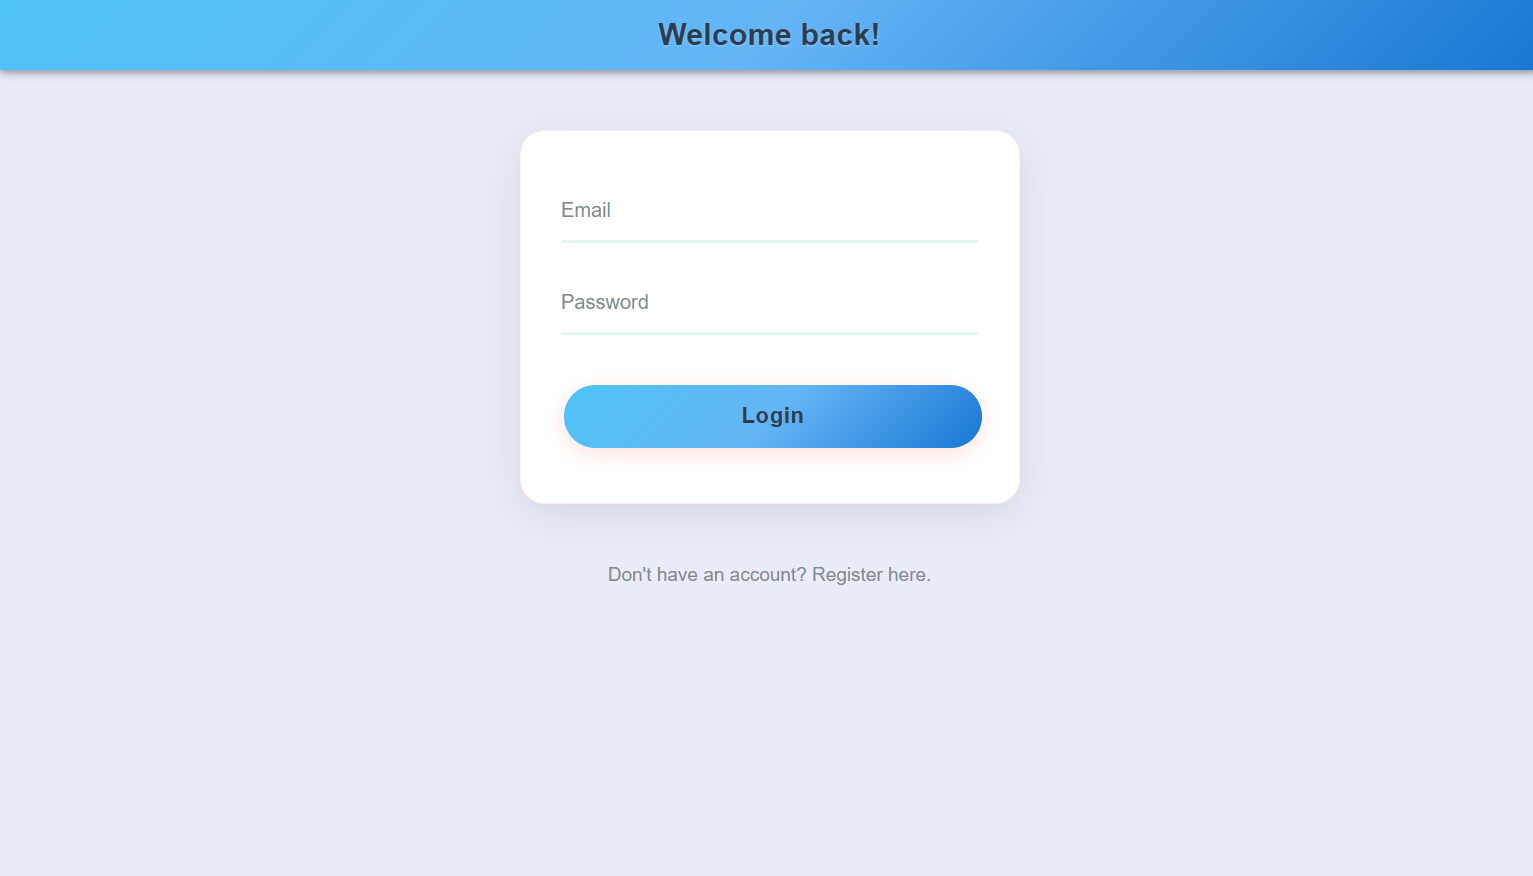
\includegraphics[scale=0.27]{./figures/login-page.png}
	\caption{Pagina de autentificare}
	\label{FigLoginPage}
\end{figure}

\par
Figura \ref{FigRegisterPage} ilustrează pagina de înregistrare, unde utilizatorul trebuie să completeze formularul cu numele, adresa de e-mail și parola.
La acționarea butonului de înregistrare, sistemul validează informațiile furnizate și creează contul utilizatorului sau afișează mesaje corespunzătoare în cazul unei erori.
După o înregistrare cu succes, user-ul este redirecționat către pagina de logare.

\begin{figure}[htbp]
	\centering
    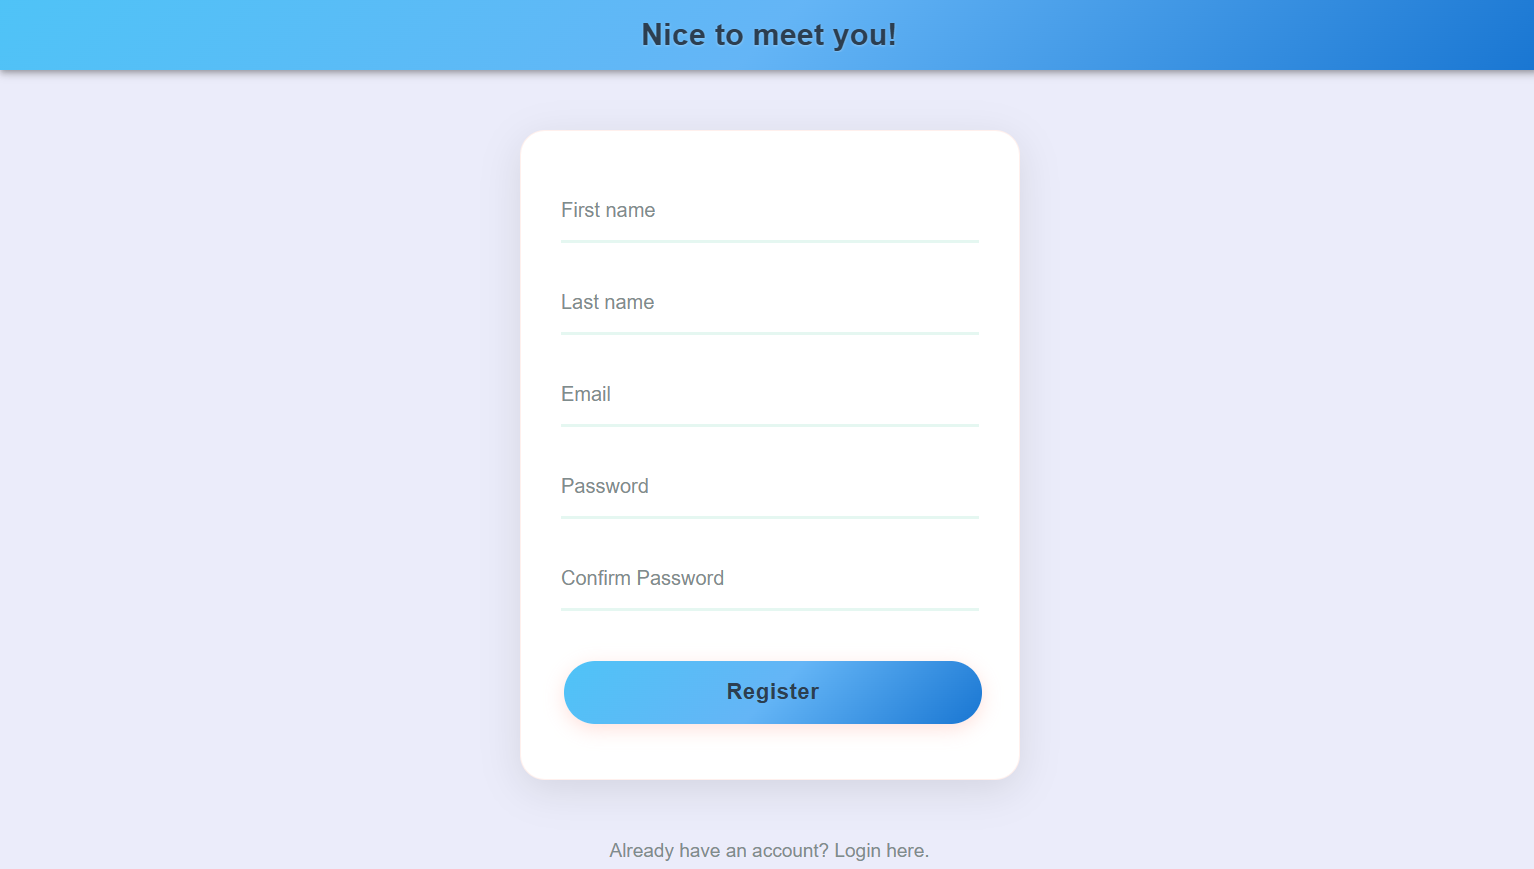
\includegraphics[scale=0.32]{./figures/register-page.png}
	\caption{Pagina de înregistrare}
	\label{FigRegisterPage}
\end{figure}

\par
În cazul în care utilizatorul logat nu are adăugate hobby-uri, un ecran dedicat acestei acțiuni va fi afișat imediat după logare, așa cum se poate observa în figura \ref{FigOnboardingPage}.
Aici user-ul poate alege din lista de hobby-uri existente, prin intermediul unui checkbox. 
De asemenea, hobby-urile pot fi filtrate după nume, folosind bara de căutare.
După selectare, acestea pot fi salvate prin apăsarea butonului Save.

\begin{figure}[htbp]
	\centering
    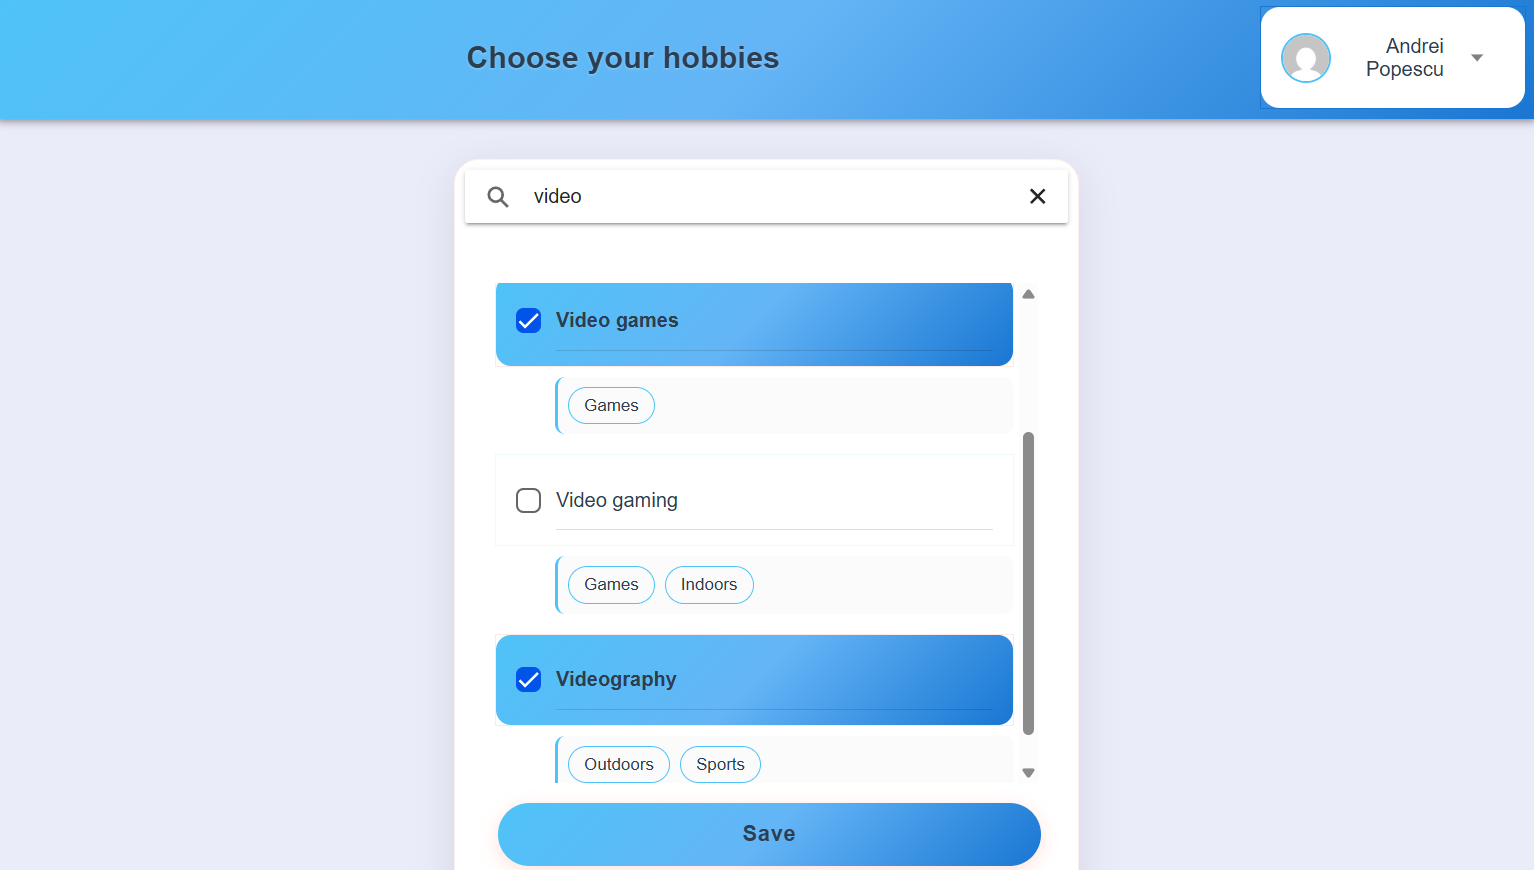
\includegraphics[scale=0.32]{./figures/onboarding-page.png}
	\caption{Pagina afișată utilizatorilor fără hobby-uri selectate}
	\label{FigOnboardingPage}
\end{figure}

\par
Dacă utilizatorul logat are hobby-uri selectate, se prezintă pagina de căutare a utilizatorilor cu hobby-uri asemănătoare, conform figurii \ref{FigHomePage}.
Pentru căutare, user-ul apasă butonul dedicat de pe ecran și se afișează lista utilizatorilor recomandați.
Această listă este ordonată descrescător după scorul potrivirii.

\begin{figure}[htbp]
	\centering
    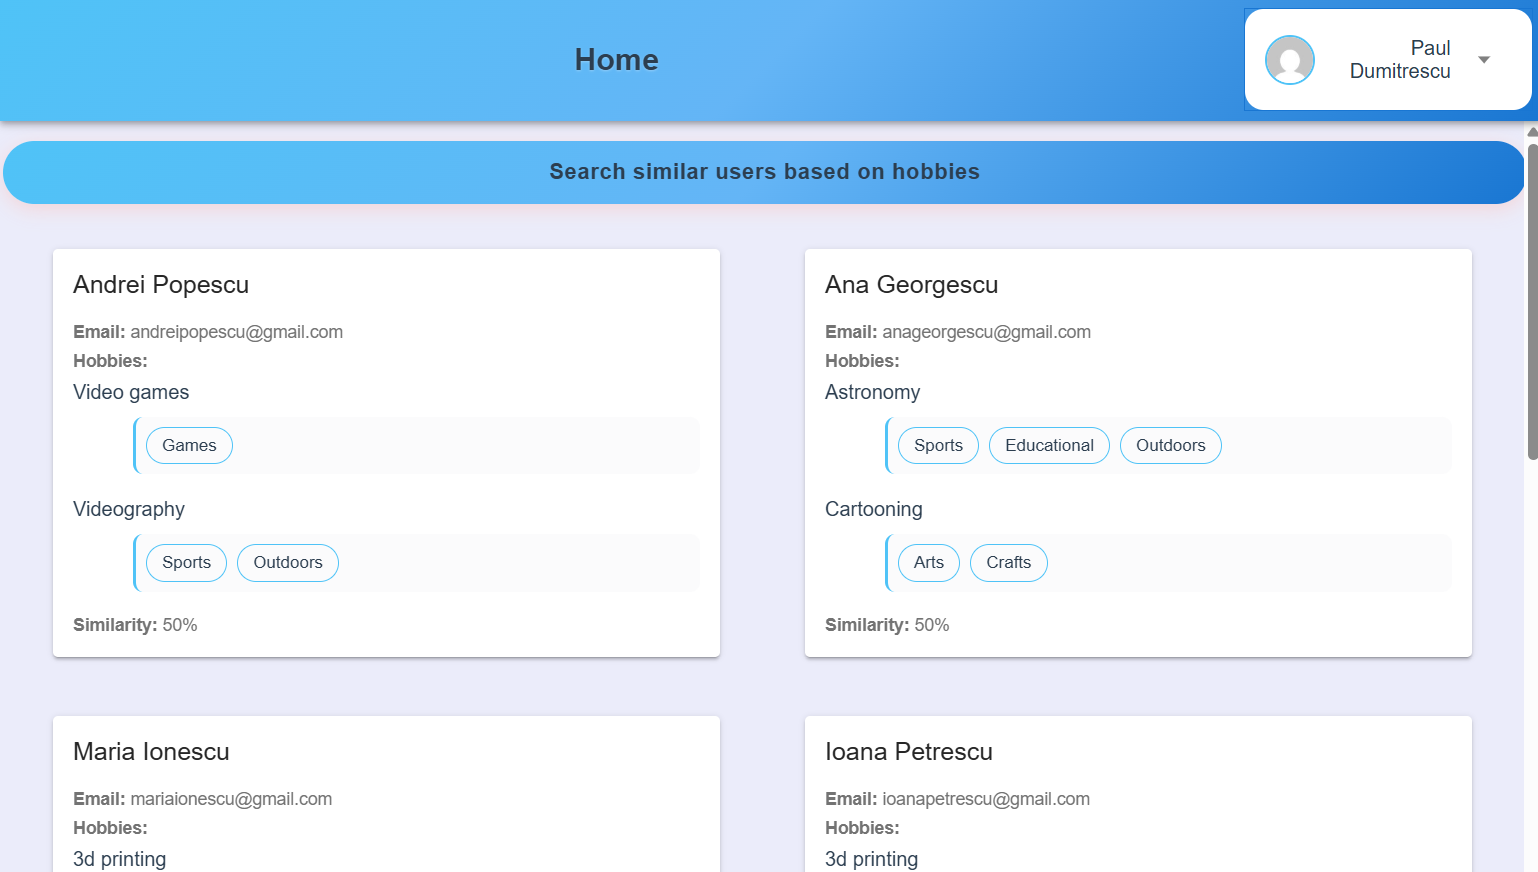
\includegraphics[scale=0.33]{./figures/home-page.png}
	\caption{Pagina de căutare a utilizatorilor cu interese comune}
	\label{FigHomePage}
\end{figure}

\par
De asemenea, utilizatorul se poate deconecta din aplicație. La apăsarea butonului ilustrat în figura \ref{FigLogoutButton}, user-ul va fi redirecționat către pagina de autentificare.

\begin{figure}[htbp]
	\centering
    
\includegraphics[scale=0.33]{./figures/logout-component.png}
	\caption{Deconectarea utilizatorului}
	\label{FigLogoutButton}
\end{figure}

\chapter{Concluzii}
\label{conclusions}

%\addcontentsline{toc}{chapter}{Concluzii}
%\addcontentsline{toc}{chapter}{Conclusions}

\bibliography{references}

\end{document}
